\documentclass{ximera}
\input{../preamble}
\addPrintStyle{..}



\begin{document}
	\author{Zomercursus KU Leuven}
	\xmtitle{Complexe getallen (meetkundige definitie)}{}
	
	\label{xim:complexe_getallen_meetkundif}

%moeten we hier over het reële vlak R2 spreken of gwn over 'het vlak' ? 

% Complexe getallen geven ons een nieuwe manier om naar het vlak te kijken. 
% Het reële vlak \(\R^2\) bestaat uit koppels \((a,b)\) waarbij \(a\) en \(b\) reële getallen zijn. 
% Zo liggen de punten \((2,1)\), \((-2,2)\) en \((0,0)\) in het reële vlak. 
% Het reële vlak wordt gekenmerkt de x-as en y-as die elkaar snijden in de oorsprong. 

% de oosprong in vb koppels zetten en als 0 +0i? 

Met complexe getallen kan je op op een nieuwe manier naar het vlak kijken. 
\\
Je weet al dat je door een $x$-as en een $y$-as in te voeren 
elk punt van het vlak met behulp van coördinaten kan schrijven als \textbf{een koppel} \((a,b)\) reële getallen.
Zo ligt bijvoorbeeld punt \((1,0)\) op de $x$-as, punt \((2,1)\) in het \textbf{eerste kwadrant}, en is \((0,0)\) de \textbf{oorsprong}.
%Het vlak wordt gekenmerkt door twee assen die elkaar snijden in de oorsprong. 
%Deze assen krijgen meestal de naam x-as en y-as, waarmee ook elk punt een x- en y-coördinaat krijgt.

%dat de assen loodrecht snijden boeit hier niet --> hoeven lln zich nu geen vragen bij te stellen. 
% op de tekening is het duidelijk 

%voor lln is het duidelijker om te spreken over 'het vlak' en het complexe vlak. 

%Wanneer het vlak bekeken wordt als voorstelling voor de complexe getallen, spreekt men over het complexe vlak. 
% Wanneer het vlak bekeken wordt als complexe getallen, spreekt men over het complexe vlak. 
% Elk punt in het (complexe) vlak stelt dan een complex getal voor. 
% Zo liggen bijvoorbeeld de complexe getallen \((2+i)\), \((-2+2i)\) en \((0+0i)\) in het vlak. 
% Het complexe vlak bestaat ook uit twee assen die elkaar snijden in de oorsprong. 


\begin{image}[0.7\textwidth]
	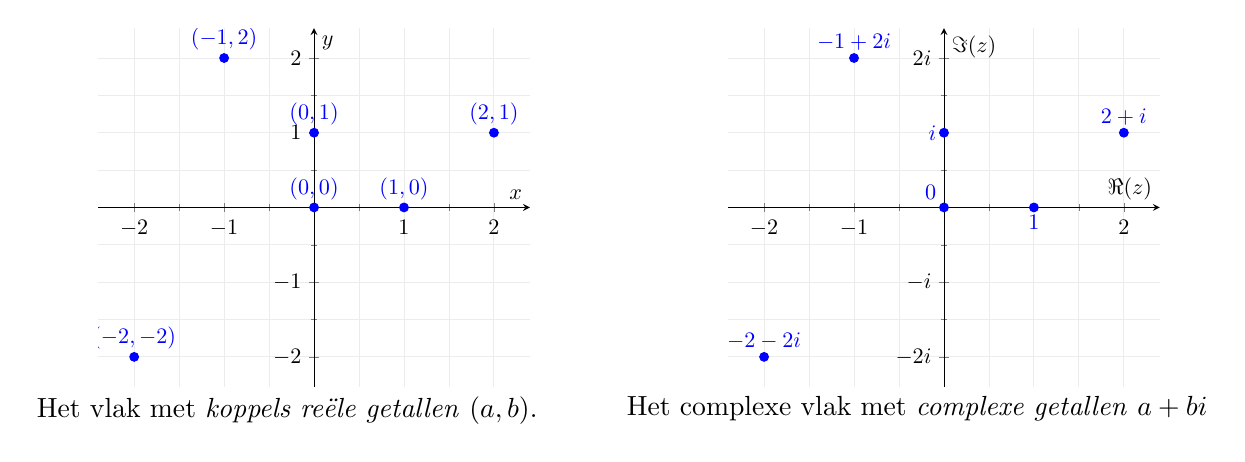
\begin{tikzpicture}[scale=0.8]
		\begin{scope}
			\begin{axis}[
				axis lines = center,
				grid=both,
				grid style={gray!15},
				minor tick num=1,
				% ticks=both,
				xlabel=$x$,
				ylabel=$y$,
				ytick ={-7,...,8}, 
				xtick ={-7,...,8}, 
				ymin=-2,ymax=+2,
				xmin=-2,xmax=+2,
				enlargelimits=true, 
				]
				
				\addplot [blue, mark = *] coordinates {( 0, 0)} node[above] {$(0,0)$};
				\addplot [blue, mark = *] coordinates {( 1, 0)} node[above] {$(1,0)$};
				\addplot [blue, mark = *] coordinates {( 0, 1)} node[above] {$(0,1)$};
				% \addplot [blue, mark = *] coordinates {( 2, 0)} node[above] {$(2,0)$};
				\addplot [blue, mark = *] coordinates {( 2, 1)} node[above] {$(2,1)$};
				\addplot [blue, mark = *] coordinates {( 2,-3)} node[above] {$(2,-3)$};
				\addplot [blue, mark = *] coordinates {(-1, 2)} node[above] {$(-1,2)$};
				\addplot [blue, mark = *] coordinates {(-2,-2)} node[above] {$(-2,-2)$};

			\end{axis}
			\node[below] at (3,0) {Het vlak met \textit{koppels reële getallen} $(a,b)$.};
		\end{scope}

		\begin{scope}[xshift=10cm]
			\begin{axis}[
				axis lines = center,
				grid=both,
				grid style={gray!15},
				minor tick num=1,
				% ticks=both,
				xlabel=$\Re(z)$,
				ylabel=$\Im(z)$,
				ytick ={-7,...,8}, yticklabels={$-7i$, $-6i$, $-5i$, $-4i$, $-3i$, $-2i$, $-i$, $0$, , $2i$, $3i$, $+3i$, $+4i$, $+5i$, $+6i$, $+7i$, $+8i$},
				xtick ={-3,...,3}, xticklabels={$-3$,$-2$,$-1$, , ,$2$,$3$},
				ymin=-2,ymax=+2,
				xmin=-2,xmax=+2,
				enlargelimits=true,
				]
				
				\addplot [blue, mark = *] coordinates {( 0, 0)} node[above left] {$0$};
				\addplot [blue, mark = *] coordinates {( 1, 0)} node[below] {$1$};
				\addplot [blue, mark = *] coordinates {( 0, 1)} node[left] {$i$};
				%\addplot [blue, mark = *] coordinates {( 2, 0)} node[above left] {$2$};
				\addplot [blue, mark = *] coordinates {( 2, 1)} node[above] {$2+i$};
				\addplot [blue, mark = *] coordinates {( 2,-3)} node[above] {$2-3i$};
				\addplot [blue, mark = *] coordinates {(-1, 2)} node[above] {$-1+2i$};
				\addplot [blue, mark = *] coordinates {(-2,-2)} node[above] {$-2-2i$};
			\end{axis}
			\node[below] at (3,0) {Het complexe vlak met \textit{complexe getallen} \(a+bi\)};
		\end{scope}
	\end{tikzpicture}
\end{image}



Door nu het punt \((0,1)\) op de $y$-as een nieuwe naam $i$ te geven, en het punt \((1,0)\) op de $x$-as gewoon als  $1$,  
kan je het punt \((2,1)\) ook schrijven als 
\[
	(2,1) = (2,0) + (0,1) = 2\cdot(1,0) + (0,1) = 2 + i
\]
en een willekeurig punt \((a,b)\) als 
\[
	(a,b) = (a,0) + (0,b) = a\cdot(1,0) + b\cdot(0,1) = a + bi
\]
Deze eenvoudige operatie lijkt op het eerste zicht misschien wat merkwaardig, maar zal blijken bijzonder interessant te zijn en een volledig nieuwe wiskundige wereld te openen met toepassingen in computerwetenschappen, fysica en ingenieurswetenschappen.
De kracht volgt vooral uit de afspraak dat $i^2=i\cdot i=-1$.

%Deze assen worden de reële-as en imaginaire-as genoemd. 

%Verder in de cursus zal duidelijk worden dat het complexe vlak vaak erg nuttig is. 

\begin{definition}[Complex getal]\label{def:complex_getal}\label{def:reeel_deel}\label{def:imaginair_deel}
	%
    Een \textbf{complex getal} is een uitdrukking van de vorm \(a+bi\), met \(a,b \in \R\)
	en $i$ een nieuw symbool waarvoor we afspreken dat \( \important{i^2=-1}\).
    %\\
    %Het symbool \(i\) waarvoor \( \important{i^2=-1}\) noemen we de \textbf{imaginaire eenheid}.
	%	
	Een complex getal \(a+bi\) kan je bekijken als een nieuwe schrijfwijze voor het punt \((a,b)\).
	De \textbf{verzameling complexe getallen} noteren we met \(\important{\C=\{a+bi \;|\; a,b\in\R;\; i^2=-1\}} \), en wordt ook het \textbf{complexe vlak} genoemd.
	% waarbij de horizontale as de \textbf{reële as} is, en de verticale de \textbf{imaginaire as}. 

	\begin{image}[0.6\textwidth]
		\begin{tikzpicture}[scale=2.5]%,cap=round,transform canvas={scale=0.5}]
			
			\tikzmath{\hoek = 35;}

			\begin{scope}
				\draw[->] (-0.1,0) -- (1.2,0) node[above] {$x$};
				\draw[->] (0,-0.1) -- (0,1)   node[right] {$y$};
				
				%    	\draw[color=blue,thick] (0:0)  -- (\hoek:1); 
				%
				\draw[color=black] (\hoek:1) node[name=P,circle, fill=black, radius=1pt,scale=0.8] {} node [yshift=2pt,above] {$(a,b)$} ;  
				%
				\draw[dashed] ({cos(\hoek)},0) node[circle, fill=black, radius=1pt,scale=0.5] {} node[below] {$a$} -- (P);
				\draw[dashed] (0,{sin(\hoek)}) node[circle, fill=black, radius=1pt,scale=0.5] {} node[left] {$b$} -- (P);
				%
				\draw [thick, red,decorate,decoration={brace,amplitude=10pt,mirror},yshift=-5pt](0,0) -- ({cos(\hoek)},0) node[black,midway,yshift=-0.6cm] {\footnotesize $a$};
				%
				\draw [thick, red,decorate,decoration={brace,amplitude=10pt},xshift=-5pt](0,0) -- (0,{sin(\hoek)}) node[black,midway,left,xshift=-8pt] {\footnotesize $b$};
			\end{scope}

			
			\begin{scope}[xshift=2cm]

			\draw[->] (-0.1,0) -- (1.2,0) node[above] {Re$(z)$};
			\draw[->] (0,-0.1) -- (0,1)   node[right] {Im$(z)$};
			
			%\draw[color=blue,thick] (0:0)  -- (\hoek:1); 
			%
			\draw[color=black] (\hoek:1) node[name=P,circle, fill=black, radius=1pt,scale=0.8] {} node [yshift=2pt,above] {$z=a+bi$} ;  
			%
			\draw[dashed] ({cos(\hoek)},0) node[circle, fill=black, radius=1pt,scale=0.5] {} node[below] {$a$} -- (P);
			\draw[dashed] (0,{sin(\hoek)}) node[circle, fill=black, radius=1pt,scale=0.5] {} node[left] {$bi$} -- (P);
			%
			\draw [thick, red,decorate,decoration={brace,amplitude=10pt,mirror},yshift=-5pt](0,0) -- ({cos(\hoek)},0) node[black,midway,yshift=-0.6cm] {\footnotesize $a$};
			%
			\draw [thick, red,decorate,decoration={brace,amplitude=10pt},xshift=-5pt](0,0) -- (0,{sin(\hoek)}) node[black,midway,left,xshift=-8pt] {\footnotesize $b$};
			
			\end{scope}
			
			
		\end{tikzpicture}
	\end{image}	
	%
	Voor  $z=a+bi$ noemen we
	\begin{tabular}{l}    
		$a$ het \textbf{reëel deel}     \\
		$b$ het \textbf{imaginair deel} \\
	\end{tabular}
	en we noteren
	\begin{tabular}{l}    
		 $\important{\Re(z)} = \Re(a+bi) = a$ \\
		 $\important{\Im(z)} = \Im(a+bi) = b$ \\
	\end{tabular}.
	
	\begin{tabular}{@{}l@{ }ll}    
		Als $\Im(z) = b=0$, dan is $z=a$ & een \textbf{(zuiver) re\"eel getal}, en  \\%& en $\R$ is dus een deelverzameling van $\C$,\\
		als $\Re(z) = a=0$, dan is $z=bi$ & een \textbf{(zuiver) imaginair getal}.
	\end{tabular}
    
\end{definition}

\begin{quickquestion*}{}
	Waar liggen de zuiver imaginaire getallen in het complexe vlak?
	% \hspace*{28mm} 
	En waar de zuiver reële getallen? 
\end{quickquestion*}

% Gelijkheid hoeft hier niet *in* de definitie, een opmerking volstaat.
Omdat complex getallen overeenkomen met punten in het vlak, zijn twee complexe getallen aan elkaar gelijk als ze dezelfde reële en imaginaire delen hebben:
\vspace{-0.35cm}
\begin{center}
	\begin{tabular}{l@{\quad}ccc}
		       & \(a+bi = c + di\) &\(\iff\)& \(a = c\) en \(b = d\)\\   
		of ook & \(z = w\)         &\(\iff\)& \(\Re(z)=\Re(w)\) en \(\Im(z)=\Im(w)\) \\    
	\end{tabular}
\end{center}


% optioneel: 

% \begin{quickquestion*}{}
% 	iets van overtuig je van de naar imaginaire EENHEID? (1,0) vs (0,1).
% \end{quickquestion*}

\begin{example} Volgende uitdrukkingen zijn allemaal complexe getallen:
$$
\def\arraystretch{1.5}
\begin{array}{c|rr c lll}
    z & \Re(z) & \Im(z) \\\hline
    2+3i & \answer{2} & \answer{3} 
    \\
    5-6i &\answer{5} & \answer{-6} 
    \\
    1+i\sqrt{2} & \answer{1} & \answer{\sqrt{2}}
    \\
    \dfrac{1-i\sqrt{5}}{2}  & \answer{\dfrac{1}{2}} & \answer{-\dfrac{\sqrt{5}}{2}}
    \\
\end{array}
\qquad\qquad
\begin{array}{c|rr c lll}
    z & \Re(z) & \Im(z) \\\hline
    1+\pi & \answer{1+\pi} & \answer{0}
    \\
    42 & \answer{42} & \answer{0}
    \\
    42i & \answer{0} & \answer{42} 
    \\
    5i + 7 & \answer{7} & \answer{5} 
    \\
    2+ 5i + \pi & \answer{2+\pi} & \answer{5} 
    \\
\end{array}
$$
De getallen $42$ en $1+\pi$ zijn zuiver reële getallen, $42i$ is een zuiver imaginair getal. 
\\
\end{example}


\begin{exercise} Geef telkens  het reëel en het imaginair deel van de volgende complexe getallen.
	\begin{xmmulticols}
	\begin{question}
		\(8+3i\)
		\begin{oplossing} \(\Re(8+3i) = 8\) en \(\Im(8+3i) = 3\)\end{oplossing}
	\end{question}
	
	\begin{question}
		\(\sqrt{2} + \sqrt{2}i\)
	\end{question}
	\begin{question}
		\(7i\)
	\end{question}
	\begin{question}
		\(\frac{1+2i}{3}\)
	\end{question}
	\begin{question}
		\(1\)
	\end{question}
	\begin{question}
	\(i\)
	\end{question}
	\begin{question}
		\(\frac{9+3i}{3}\)
	\end{question}
	\begin{question}
		\(\pi + e + i \)
	\end{question}
	\begin{question}
		\(0\)
	\end{question}
	\begin{question}
		\(\frac{\sqrt{5} + \sqrt{5}i }{\sqrt{5}}\)
	\end{question}
	
	\end{xmmulticols}
	
\end{exercise}
	
\begin{exercise} Schrijf zo eenvoudig mogelijk, door gebruik te maken van de gelijkheid $i^2=-1$.
	\begin{xmmulticols}[5]
	\begin{question}
		\(i^2\)
	\end{question}
	\begin{question}
		\(i^5\)
	\end{question}
	\begin{question}
		\(-i^3\)
	\end{question}
	\begin{question}
		\(i^4\)
	\end{question}
	\begin{question}
		\(-i^4\)
	\end{question}
	\begin{question}
		\(i^{10}\)
	\end{question}
	\begin{question}
		\(i^{11}\)
	\end{question}
	\begin{question}
		\(-i^{12}\)
	\end{question}
	\begin{question}
		\(-i^2\)
	\end{question}
	\begin{question}
		\(-i^3\)
	\end{question}
	\end{xmmulticols}
\end{exercise}
	
% \begin{exercise}{Ga na of de volgende complexe getallen aan elkaar gelijk zijn.}
% 	\begin{xmmulticols}
	
% 	\begin{question}
% 		\(\) en \(\)
% 	\end{question}
% 	\begin{question}
% 		\(\) en \(\)
% 	\end{question}
% 	\begin{question}
% 		\(\) en \(\)
% 	\end{question}
% 	\begin{question}
% 		\(\) en \(\)
% 	\end{question}
% 	\begin{question}
% 		\(\) en \(\)
% 	\end{question}
% 	\begin{question}
% 		\(\) en \(\)
% 	\end{question}
% 	\begin{question}
% 		\(\) en \(\)
% 	\end{question}
% 	\begin{question}
% 		\(\) en \(\)
% 	\end{question}
% 	\begin{question}
% 		\(\) en \(\)
% 	\end{question}
% 	\begin{question}
% 		\(\) en \(\)
% 	\end{question}
% 	\begin{question}
% 		\(\) en \(\)
% 	\end{question}
% 	\end{xmmulticols}
% \end{exercise}

\end{document}

